%%%%%%%%%%%%%%%%%%%%%%%%%%%%%%%%%%%%%%%%%%%%%%%%%%%%%%%%%%%%%%%%%%%%%%%%%%%%%%%%
%2345678901234567890123456789012345678901234567890123456789012345678901234567890
%        1         2         3         4         5         6         7         8

%\documentclass[letterpaper, 10 pt, conference]{ieeeconf}  % Comment this line out if you need a4paper

\documentclass[letterpaper, 10pt, conference]{ieeeconf}      % Use this line for a4 paper

\IEEEoverridecommandlockouts                              % This command is only needed if 
                                                          % you want to use the \thanks command

\overrideIEEEmargins                                      % Needed to meet printer requirements.

% See the \addtolength command later in the file to balance the column lengths
% on the last page of the document

% The following packages can be found on http:\\www.ctan.org
\usepackage{graphicx} % for pdf, bitmapped graphics files
%\usepackage{epsfig} % for postscript graphics files
%\usepackage{mathptmx} % assumes new font selection scheme installed
%\usepackage{times} % assumes new font selection scheme installed
\usepackage{amsmath} % assumes amsmath package installed
%\usepackage{amssymb}  % assumes amsmath package installed
\usepackage{subfigure}
\bibliographystyle{IEEEtran}

\title{\LARGE \bf
**
}


\author{
**%
\thanks{
**}	
	}




\begin{document}



\maketitle
\thispagestyle{empty}
\pagestyle{empty}


%%%%%%%%%%%%%%%%%%%%%%%%%%%%%%%%%%%%%%%%%%%%%%%%%%%%%%%%%%%%%%%%%%%%%%%%%%%%%%%%
\begin{abstract}

**
\end{abstract}




%%%%%%%%%%%%%%%%%%%%%%%%%%%%%%%%%%%%%%%%%%%%%%%%%%%%%%%%%%%%%%%%%%%%%%%%%%%%%%%%
\section{INTRODUCTION}

It has become a commonplace for the  bipedal robots to share environments with humans and provide assistance in complex tasks. Although, their ability to cope with changing, unstructured environments remains un-honed: for instance, walking on uneven terrains seems like an arduous task. While a part of this challenge lies in controlling the system dynamically depending on the input wrenches acting on the system, the other focuses in estimating these quantities accurately in order to provide a proper feedback. We seek for a versatile system which can adapt to the changing terrains and feed proper estimates of the wrenches acting on the system to the controller. Unlike on rigid surfaces, balancing or walking on a compliant surface is quite different in which case accurate estimation of the orientation and the wrenches on the foot becomes essential. While walking on slippery surfaces, we are not always aware of the forces that are exerted on the foot in order to make a proper contact. Hence, we need to adaptively estimate these constraint forces between the foot of the biped and the compliant surface. 

The survey on non-linear estimation methods reported in [1] informs us of the popular technique of Adaptive Extended Kalman Filtering used to estimate the unknown parameters of a non-linear dynamic system. The technique of parameter estimation is widely applied in the space-crafts to simultaneously estimate the attitude along with the dynamic parameters of the space-craft, either by using least square methods or by modelling the unknown parameters using polynomials in time as basis functions, [2][3][4][5]. In [6], [7] and [8], the authors explain the dual estimation problem of estimating simultaneously states and parameters of a dynamic system, given the noisy measurements, which can be applied in adaptive control where the parameters are used in design process and estimated states are used for feedbacks. Two approaches of the dual estimation problem are proposed: 1. Joint State and Parameter Estimation, where states and parameters are combined in a joint bilinear state-space representation. 2. Dual State and Parameter Estimation, where two filters, each for state and parameter, are run simultaneously, and the current parameter estimate is used by state filter and vice-versa. The dual estimation method is simplistic, has a low computation cost and provides good convergence and robust estimates.


In this paper, we propose a framework to implement and test the dual estimation based algorithms for foot posture and contact force estimation for bipedal robots. Assuming the foot to be a single rigid body, it is subject to the wrenches due to contacts $(f_c,\mu_c)$, wrenches due to the rest of the body $(f_o,\mu_o)$, and the forces due to gravity as a function of the orientation of the foot. Additionally, we incorporate a virtual torsional spring, to model the contact forces, whose stiffness will vary adaptively depending on the rigidity of the surface. Hence estimating the parameters of the stiffness matrix gives us the knowledge of the compliant characteristic of the contact made by the biped with the surface.


\subsection{DEKF}

Used to estimate both state and model  from only noisy measurements. Two EKFs are run concurrently : At every time step, the state filter estimates the state using the current model estimate $\hat{x}_{k+1}$, while the parameter filter estimates the parameters using current state estimate $\hat{x}_{k+1}$
The estimate and covariances of the state and the parameter are initialised as,
	$$\hat{w}_{0} = E[w] ; 	P_{w_{0}} = E[(w - \hat{w}_{0})(w - \hat{w}_{0})^{T}]$$
	$$\hat{x}_{0} = E[x] ; 	P_{x_{0}} = E[(x - \hat{x}_{0})(x - \hat{x}_{0})^{T}]$$
	
The time-update equations are the following,\linebreak
\textit{	Prediction:} 
\linebreak
\textit{Parameter filter:}
  $$\hat{w}_{k+1}^{-} = \hat{w}_{k}$$
  $$P_{w_{k+1}}^{-} = P_{w_{k}} + Q_{k}^{w} = \lambda^{-1}P_{w_{k}}$$
  where $\lambda$ is a forgetting factor with values in the range of (0,1].
\linebreak
\textit{State filter:}
  $$\hat{x}_{k+1}^{-} = f(\hat{x}_{k}^{+},u_{k},\hat{w}_{k+1}^{-})$$
$$P_{x_{k+1}}^{-} = F_{k}P_{x_{k}}^{+}F_{k}^{T} + Q_{k}^{x} $$
\linebreak
The measurement-update equations are given by,
\linebreak
\textit{	Update:} 
\linebreak
\textit{State filter:}
$$K^{x}_{k+1} = P_{x_{k+1}}^{-}H_{k+1}^{T}(H_{k+1}P_{x_{k+1}}^{-}H_{k+1}^{T} + R_{k+1}^{x})^{-1} $$
$$\hat{x}_{k+1}^{+} = \hat{x}_{k+1}^{-} + K^{x}_{k+1}(y_{k+1} - h(\hat{x}_{k+1}^{-})) $$
$$P_{x_{k+1}}^{+} = (I-K^{x}_{k+1}H_{k+1})P_{x_{k+1}}^{-}$$

\textit{Parameter filter:}
$$\hat{w}_{k+1}^{+} = \hat{w}_{k+1}^{-} + K^{w}_{k+1}(y_{k+1} - h(\hat{x}_{k+1}^{-})) $$

$$K^{w}_{k+1} = P_{w_{k+1}}^{-}C_{k+1}^{T}(C_{k+1}P_{w_{k+1}}^{-}C_{k+1}^{T} + R_{k+1}^{w})^{-1} $$

$$P_{w_{k+1}}^{+} = (I-K^{w}_{k+1}C_{k+1})P_{w_{k+1}}^{-}$$

The Jacobian matrices are defined as follows,
$$F_{k} = \frac{\partial f(x,\hat{w}_{k+1}^{-})}{\partial x}\bigg|_{\hat{x}_{k}^{+}} ; H_{k} = \frac{\partial h(x)}{\partial x}\bigg|_{\hat{x}_{k+1}^{-}} $$
$$ C_{k} = \frac{\partial h(\hat{x}_{k+1}^{-})}{\partial w} = H_{k+1}\frac{\partial \hat{x}_{k+1}^{-}}{\partial w}\bigg|_{\hat{w}_{k+1}^{-}} $$
\linebreak

The linearisation associated with the Parameter filter is defined in such a way because the state filter whose parameters are estimated by the parameter filter, has a recurrent architecture, i.e., $\hat{x}_{k+1}$ is a function of $\hat{x}_{k}$, and both are functions of w. Thus the linearisation must be computed using recurrent derivatives. The author specifies a routine similar to real-time recurrent learning for the linearisation., for further reading : look into [6]. 
%\subsection{JEKF}
%The unknown parameters $w$ are considered as additional state variables, hence we have an augmented state vector,
%$$z = [x^{T} \theta^{T}]^{T}$$
%
%$$ z_{k+1} = \begin{pmatrix}x_{k+1}\\\theta_{k+1}\end{pmatrix} = \begin{pmatrix}f(x_{k},u_{k},\theta_{k})\\\theta_{k}\end{pmatrix} + \begin{pmatrix}w_{k}\\\eta_{k}\end{pmatrix}$$

\subsection{JEKF}

\subsection{Proper computation of wrenches on the foot}

Currently,we consider the leg as a single rigid body and assume the wrenches act at the COM of the whole leg, i.e., at the knee of the leg. But it would be interesting to considering the wrenches acting exclusively  on the foot for obtaining accurate estimates. Hence the following equations show the Newton-Euler equations for the wrenches acting on the foot:



For this purpose we consider three link bodies $b_{0}$ : foot,  $b_{1}$ : lower leg , $b_{1}$ : upper leg.
\linebreak
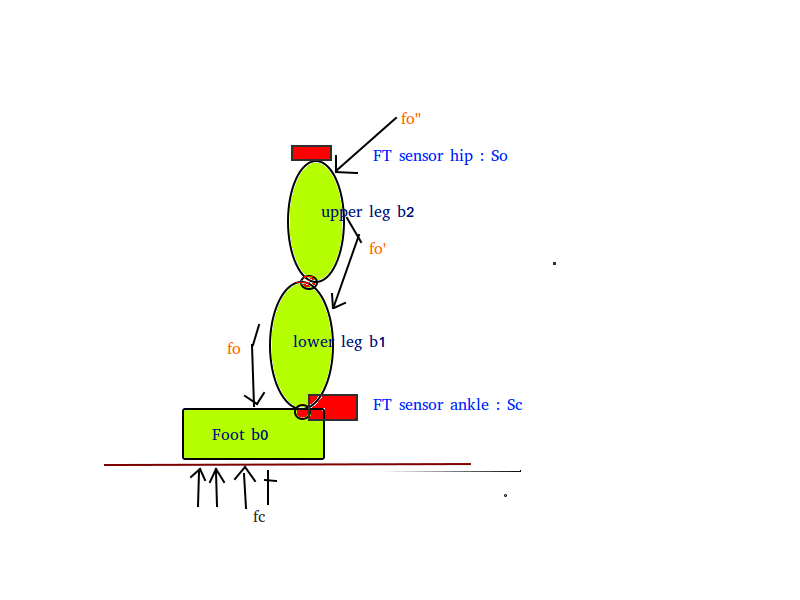
\includegraphics[scale = 0.25]{legmodel}
\linebreak
Excuse me for the bad figure :P
\linebreak
Let's consider only the foot ,body $b_{0}$. The wrenches acting on the foot are the ground reaction wrenches due to contact $f_{c}$, wrenches from the  rest of the body $f_{o}$ and wrenches due to gravity. Hence ,

$$ f_{o} - f_{c}  + I^{b_{0}}g^{b_{0}} = I^{b_{0}}a^{b_{0}} + v^{b_{0}}\times (I^{b_{0}}v^{b_{0}}) $$

Similarly, the wrenches acting on the lower leg, body $b_{1}$ are $f_{o}$ and $f_{o}^{'}$ and those acting on the upper leg, body $b_{2}$ are $f_{o}^{'}$ and $f_{o}^{''}$.

$$ f_{o}^{'} - f_{o}  + I^{b_{1}}g^{b_{1}} = I^{b_{1}}a^{b_{1}} + v^{b_{1}}\times (I^{b_{1}}v^{b_{1}}) $$

$$ f_{o}^{''} - f_{o}^{'}  + I^{b_{2}}g^{b_{2}} = I^{b_{2}}a^{b_{2}} + v^{b_{2}}\times (I^{b_{2}}v^{b_{2}}) $$

This has a recursive structure, and hence can easily be obtained using the RNEA algorithm, which is applicable for articulated structures as well.

Hence, from the above equations, we obtain, 

$$ f_{o}^{''} - f_{c} + \sum_{i=1}^{3} I^{b_{i}}g^{b_{i}} = \sum_{i=1}^{3} I^{b_{i}}a^{b_{i}} + v^{b_{i}}\times (I^{b_{i}}v^{b_{i}})$$

The forces $f_{o}^{''}$ and $f_{c}$ are measured from the FT sensors located at the hip and the ankle respectively, and are associated with the sensor frames $S_{o}$ and $S_{c}$.

When expressed in the foot frame,
$$ X^{b_{o}*}_{S_{o}} f_{o}^{''} - X^{b_{o}*}_{S_{c}} f_{c} + X^{b_{o}*}_{b_{i}} \sum_{i=1}^{3} I^{b_{i}}g^{b_{i}} = X^{b_{o}*}_{b_{i}} \sum_{i=1}^{3} I^{b_{i}}a^{b_{i}} + v^{b_{i}}\times (I^{b_{i}}v^{b_{i}})$$


In the implementation point of view, the transformation and inertia matrices can be obtained using mexWholebody model and urdf of the robots. We need to figure a way to determine the link velocities, accelerations and the gravities acting on the links.

\addtolength{\textheight}{-12cm}   % This command serves to balance the column lengths
                                  % on the last page of the document manually. It shortens
                                  % the textheight of the last page by a suitable amount.
                                  % This command does not take effect until the next page
                                  % so it should come on the page before the last. Make
                                  % sure that you do not shorten the textheight too much.

%%%%%%%%%%%%%%%%%%%%%%%%%%%%%%%%%%%%%%%%%%%%%%%%%%%%%%%%%%%%%%%%%%%%%%%%%%%%%%%%



%%%%%%%%%%%%%%%%%%%%%%%%%%%%%%%%%%%%%%%%%%%%%%%%%%%%%%%%%%%%%%%%%%%%%%%%%%%%%%%%



%%%%%%%%%%%%%%%%%%%%%%%%%%%%%%%%%%%%%%%%%%%%%%%%%%%%%%%%%%%%%%%%%%%%%%%%%%%%%%%%






%%%%%%%%%%%%%%%%%%%%%%%%%%%%%%%%%%%%%%%%%%%%%%%%%%%%%%%%%%%%%%%%%%%%%%%%%%%%%%%%





\begin{thebibliography}{99}

\bibitem{c1} A Survey of Non-Linear Attitude Estimation Methods

\bibitem{c2} Parameter Estimation of a Spacecraft Simulator Using Parameter-Adaptive Control

\bibitem{c3} Spacecraft Inertia Estimation Via Constrained Least Squares

\bibitem{c4} Dual attitude and parameter estimation of passively magnetically stabilized nano satellites


\bibitem{c5} Estimation of a Spacecraft's Attitude Dynamics Parameters by Using Flight Data

\bibitem{c6} Kalman filtering and Neural Networks, Ch5 Dual Extended Kalman Filter Methods

\bibitem{c7} Joint State and Parameter Estimation For Biochemical Dynamic Pathways With Iterative Extended Kalman Filter: Comparison With Dual State and
Parameter Estimation

\bibitem{c8} Extended Kalman Filter for Estimation of Parameters in Nonlinear State-Space Models of Biochemical Networks
\end{thebibliography}




\end{document}
















